\begin{frame}
    \frametitle{Introduction}
    \begin{columns}[T]
        \begin{column}{.48\textwidth}
            \begin{figure}[H]
                
\includegraphics[width=\textwidth]{images/performance.jpg}
                \label{fig:performance}
            \end{figure}
        \end{column}
        \hfill
        \begin{column}{.48\textwidth}
            \begin{block}{}
                Ensurance of the quality and testing of the software products. 
            \end{block}
            \begin{itemize}
                \item<1-> Continuous integration and deployment.
            \end{itemize}
        \end{column}
    \end{columns}
\end{frame}

\begin{frame}
    \frametitle{Introduction}
    \begin{columns}[T]
        \begin{column}{.48\textwidth}
            \begin{figure}[H]
                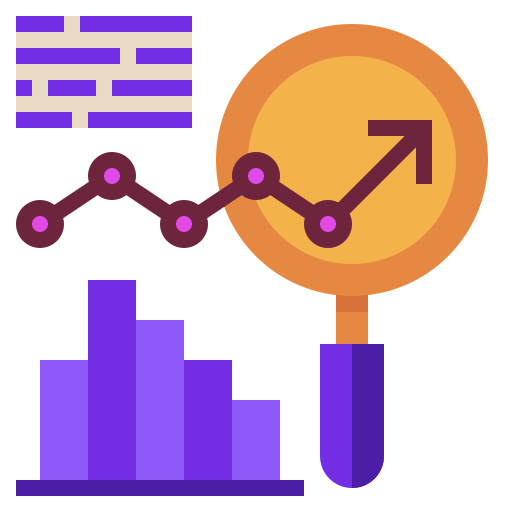
\includegraphics[width=\textwidth]{images/benchmark.png}
                \label{fig:benchmark}
            \end{figure}
        \end{column}
        \hfill
        \begin{column}{.48\textwidth}
            \begin{block}{Testing the performance}
                 Benchmarks
            \end{block}
            \begin{itemize}
                \item<2-> Scenarios
                \item<3-> Performance evaluation criteria
                \item<4-> Benchmarking score
            \end{itemize}
        \end{column}
    \end{columns}
\end{frame}

\begin{frame}
    \frametitle{Introduction}
    \begin{columns}[T]
        \begin{column}{.48\textwidth}
            \begin{figure}[H]
                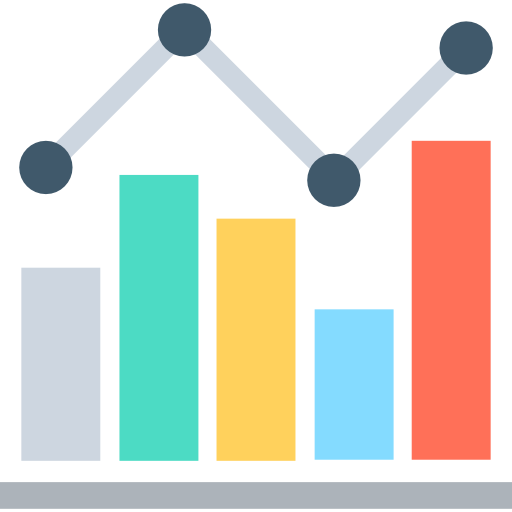
\includegraphics[width=\textwidth]{images/comparison.png}
                \label{fig:comparison}
            \end{figure}
        \end{column}
        \hfill
        \begin{column}{.48\textwidth}
            \begin{block}{Meaningful Data}
                Generated benchmark values
            \end{block}
            \begin{itemize}
                \item<2-> Understanding the performance of the system.
                \item<3-> Enabling fair comparison between different solutions.
                \item<4-> Ensuring the improvement of the system.
            \end{itemize}
        \end{column}
    \end{columns}
\end{frame}

\begin{frame}
    \frametitle{Introduction}
    \begin{columns}[T]
        \begin{column}{.48\textwidth}
            \begin{figure}[H]
                
\includegraphics[width=\textwidth]{images/infographic.png}
                \label{fig:infographic}
            \end{figure}
        \end{column}
        \hfill
        \begin{column}{.48\textwidth}
            \begin{block}{A picture is worth a thousand words}
                Data visualization
            \end{block}
            \begin{itemize}
                \item<2-> Tidious task.
                \item<3-> Can be hard.
                \item<4-> If done properly can be helpful.
            \end{itemize}
        \end{column}
    \end{columns}
\end{frame}

